\documentclass{book}
\usepackage{wrapfig}
\usepackage{graphicx}
\usepackage[table]{xcolor}
\usepackage{tikz-timing}
\usepackage{tikz}
\usetikzlibrary{shapes.geometric, arrows}
\usepackage{pgfplotstable}
\usepackage{rotating}
\usepackage{listings}
%\usepackage{biblatex}
%\addbibresource{mainframe.bib}
\begin{document}

%tikz declartions for flowchart
\tikzstyle{startstop} = [rectangle, rounded corners, minimum width=3cm, minimum height=1cm,text centered, draw=black, fill=red!30]
\tikzstyle{io} = [trapezium, trapezium left angle=70, trapezium right angle=110, minimum width=3cm, minimum height=1cm, text centered, draw=black, fill=blue!30]
\tikzstyle{process} = [rectangle, minimum width=3cm, minimum height=1cm, text centered, text width=3cm, draw=black, fill=orange!30]
\tikzstyle{decision} = [diamond, minimum width=3cm, minimum height=1cm, text centered, draw=black, fill=green!30]
\tikzstyle{arrow} = [thick,->,>=stealth]

\frontmatter
\title{Documentation for z80 Mainframe}
\author{Colton Beck}
\maketitle
\section*{Legal Information}
\subsection*{Disclaimer of Warranty}

  THERE IS NO WARRANTY FOR THE PROGRAM, TO THE EXTENT PERMITTED BY
APPLICABLE LAW.  EXCEPT WHEN OTHERWISE STATED IN WRITING THE COPYRIGHT
HOLDERS AND/OR OTHER PARTIES PROVIDE THE PROGRAM "AS IS" WITHOUT WARRANTY
OF ANY KIND, EITHER EXPRESSED OR IMPLIED, INCLUDING, BUT NOT LIMITED TO,
THE IMPLIED WARRANTIES OF MERCHANTABILITY AND FITNESS FOR A PARTICULAR
PURPOSE.  THE ENTIRE RISK AS TO THE QUALITY AND PERFORMANCE OF THE PROGRAM
IS WITH YOU.  SHOULD THE PROGRAM PROVE DEFECTIVE, YOU ASSUME THE COST OF
ALL NECESSARY SERVICING, REPAIR OR CORRECTION.

\subsection*{Limitation of Liability}

  IN NO EVENT UNLESS REQUIRED BY APPLICABLE LAW OR AGREED TO IN WRITING
WILL ANY COPYRIGHT HOLDER, OR ANY OTHER PARTY WHO MODIFIES AND/OR CONVEYS
THE PROGRAM AS PERMITTED ABOVE, BE LIABLE TO YOU FOR DAMAGES, INCLUDING ANY
GENERAL, SPECIAL, INCIDENTAL OR CONSEQUENTIAL DAMAGES ARISING OUT OF THE
USE OR INABILITY TO USE THE PROGRAM (INCLUDING BUT NOT LIMITED TO LOSS OF
DATA OR DATA BEING RENDERED INACCURATE OR LOSSES SUSTAINED BY YOU OR THIRD
PARTIES OR A FAILURE OF THE PROGRAM TO OPERATE WITH ANY OTHER PROGRAMS),
EVEN IF SUCH HOLDER OR OTHER PARTY HAS BEEN ADVISED OF THE POSSIBILITY OF
SUCH DAMAGES.
\subsection*{Fonts}
This was typeset in Computer Modern using pdf\LaTeX{} and bib\TeX{}.
The timing diagrams were made with the tikz-timing package.
The code listings were made with the listings package
\chapter*{Dedication}
Dedicated to caffeine for giving me the energy to write this and sleep deprivation for making me think this was a good idea.
\tableofcontents
\listoffigures
\listoftables
\mainmatter
\chapter{General Construction}
\section{Power Supply}
The system is designed to use one power supply to provide the low voltage for the peripherals and main board. For the system as shown here, the supply 
should be rated at least 7 amperes at 5 volts and 15 amperes at 12 volts for a combined 215 watts of total power. If additional peripherals are expected to 
be added, then the power supply should be of a higher wattage so that the whole system can be powered from a unified supply to avoid the risk of ground 
loops that could induce excessive noise.

\section{Physical Connections}
\subsection{Power}
For the rear panel power connections, any connectors may be used as long as they have sufficient current capacity for the load expected. For my design, I 
elected to use 3-pin XLR connectors as listed in Appendix B.7. If XLR connectors are used for power, they should be marked as such to avoid any 
accidental damage. The system is designed such that the power is daisy-chained from one preipheral to the next. This does mean that the total power 
draw for the whole system needs to be taken into consideration when selecting a connector type to use.

\subsection{Data}
For the data connections, the sytem is designed to use 8p8c modular connectors along with cat 5 cable for the differential connection. If a different cable is 
used, the termination resistors on the peripherals need to be changed to be of a suitable value to prevent ringing. The system is designed such that the 
data is daisy-chained from one preipheral to the next. This has the advantage that termination resistors only need to be used on the first and last device in 
the chain as specified on pg. 12 of the PCA9615 datasheet\cite{nxp:pca9615}.

\begin{wrapfigure}{R}{0.5\textwidth}
  \begin{center}
    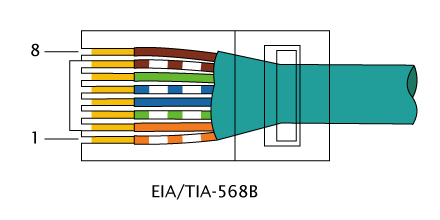
\includegraphics[width=0.48\textwidth]{RJ-45_TIA-568B_Left.png}
  \end{center}
  \caption[Example wiring using EIA-568B]{Example wiring using EIA-568B\cite{img:eia568}\label{fig:eia568}}
\end{wrapfigure}

\begin{table}
\centering
\begin{tabular}{| l | l | l |}
Pin Number & Function & Wire Color\\
1 & Data- & White/Orange\\
2 & Data+ & Orange\\
3 & NC & White/Green\\
4 & NC & Blue\\
5 & NC & White/Blue\\
6 & NC & Green\\
7 & Clock- & White/Brown\\
8 & Clock+ & Brown\\
\end{tabular}
\caption{Interface Pin Functions\label{tab:intpin}}
\end{table}
\section{Interface}
The inter-peripheral communication is done via differental I$^2$C running at 400kbit/s. This link is designed to be wired as illustrated in figure 
\ref{fig:eia568} and in table \ref{tab:intpin}. Using a parallel connection would allow for a higher throughput and would simplify some of the design 
however this comes at a higher cost due to the connectors and cabling. A circuit, shown in figure \ref{fig:intdecode}, is used to identify when a peripheral 
is being addressed and triggers a wait for the z80 and notifies a PIC that there is data ready to transmit. This portion of the circuit is designed to be 
modular since one copy is needed for each peripheral that is to be addressed and is expandable through stackable modules, shown in figure \ref{fig:decpcb}.

The z80 mainframe was designed to be modular and expandable. It accomplishes this by having a simple interface that either reads  or writes data using DMA. The system is limited to 128 connected peripherals because of the limitation of I$^2$C's 7-bit addresses.

The interface PIC(U?? in appendix C.3) is designed to look for specific addresses after which the it pulls the BUSREQ line low and reads from 0x0800 to 0x084F or writes to 0x850 to 0x089F. The peripherals listed here are designed to be configurable as to what address they respond to and the OS is configurable for where it is trying to address these devices at. Both are configured in hardware rather than in software to simplify configuration so the OS can determine settings without the ROM needing to be modified to be installation dependent.

\section{Configuration}
The system is configured through DIP switches for the addresses that the peripherals described here are located at.

\chapter{Main Board}
\section{ROM}
The ROM, listed in appendix A.1, is intended to function as a bootstrap script to prepare the system to load a program from another medium. It also serves to provide callable funtions for the default peripherals to ease implimentation in programs.

\chapter{Front Panel}
The front panel connects directly to the main board through a 36 pin header that caries the 16-bit address bus, the 8-bit data bus, power, and the 10 
control lines; BUSREQ, BUSACK, WAIT, MREQ, IORQ, RD, WR, M1, HALT, and RESET. It is designed with status LEDs for the control lines and buses as well 
as hexadecimal readouts for the buses. The front panel also includes the circuitry for an instruction single stepping circuit along with halt and reset 
controls. There also are four 8-bit inputs and four 8-bit outputs.
\section{Outputs}
\section{Inputs}

\chapter{CGA Terminal}

\chapter{Dot Matrix Printer}
The main output for the z80 mainframe is the printer. This particular setup is designed to use an Epson LX-810 printer interfacing over a parallel port as 
shown in figure~\ref{fig:printer}.

\begin{figure}[h]
\centering
\begin{tikztimingtable}
$\mathrm{DATA\:0-7}$         &   UU7D{\textnormal{MEM 0x0800}}7D{\textnormal{MEM 0x0801}}XX7D{\textnormal{MEM 0x0850}}7D{\textnormal{0x0D}}UU\\
$\overline{\mathrm{STROBE}}$ &   HHHLHHHHHHLHHHHHXXHLHHHHHHLHHHHHHH\\
$\overline{\mathrm{BUSY}}$   &   HHHHHHHHLHHHHHHLXXHHHHHHLHHHHHHLHH\\
\end{tikztimingtable}
\caption{Driver Board to Printer Timing}
\label{fig:lpttiming}
\end{figure}

\begin{figure}[h]
\centering
\begin{tikztimingtable}
$\mathrm{ADDR\:0-15}$          &   U8D{\textnormal{0x00FB}}UU6D{\textnormal{0x0800}}XXX6D{\textnormal{0x0850}}UUUU\\
$\mathrm{DATA\:0-7}$           &   UU7D{\textnormal{Option Byte}}UUXX4D{\textnormal{Data}}XXXXX4D{\textnormal{In}}UUUU\\
$\overline{\mathrm{WAIT}}$    &   UUUULLLLHHHHHHHHHHHHHHHHHHHHHU\\
$\overline{\mathrm{MREQ}}$    &   UHHHHHHHHHHHLLLLLHXXHLLLLLHHHU\\
$\overline{\mathrm{IORQ}}$    &   UHHLLLLHHHHHHHHHHHHHHHHHHHHHHU\\
$\overline{\mathrm{RD}}$      &   UHHHHHHHHHHHLLLLLHXXHLLLLLHHHU\\
$\overline{\mathrm{WR}}$      &   UHHLLLLHHHHHHHHHHHHHHHHHHHHHHU\\ 
$\overline{\mathrm{BUSREQ}}$  &   UHHHHHLLLLLLLLLLLLLLLLLLLLLHHH\\
$\overline{\mathrm{BUSACK}}$  &   UHHHHHHLLLLLLLLLLLLLLLLLLLLLHH\\
\extracode
\begin{pgfonlayer}{background}
\vertlines[help lines]{1,2,3,4,5,6,7,8,9,10,11,12,13,14,15,16,17,18,19,20,21,22,23,24,25,26,27,28,29,30}
\end{pgfonlayer}
\end{tikztimingtable}
\caption{Main Bus to Printer Driver Timing}
\label{fig:lptdrivertiming}
\end{figure}

\begin{figure}[h]
\begin{tikzpicture}[node distance=2cm]
\node (start) [startstop] {Start};
\node (in1) [io, below of=start] {Input};
\node (pro1) [process, below of=in1] {Process 1};
\node (dec1) [decision, below of=pro1, yshift=-0.5cm] {Decision 1};
\node (pro2a) [process, below of=dec1, yshift=-0.5cm] {Process 2a};
\node (pro2b) [process, right of=dec1, xshift=2cm] {Process 2b};
\node (out1) [io, below of=pro2a] {Output};
\node (stop) [startstop, below of=out1] {Stop};
\draw [arrow] (start) -- (in1);
\draw [arrow] (in1) -- (pro1);
\draw [arrow] (pro1) -- (dec1);
\draw [arrow] (dec1) -- node[anchor=east] {yes} (pro2a);
\draw [arrow] (dec1) -- node[anchor=south] {no} (pro2b);
\draw [arrow] (pro2b) |- (pro1);
\draw [arrow] (pro2a) -- (out1);
\draw [arrow] (out1) -- (stop);
\end{tikzpicture}
\caption{Code Flowchart}
\label{fig:lptcodeflow}
\end{figure}

\chapter{Card Punch \& Reader}

\chapter{Paper Tape Punch \& Reader}

\appendix
\chapter{Code Listings}
\lstset{numbers=left, numberstyle=\tiny, stepnumber=1, numbersep=5pt}
\section{ROM Listing}
\cleardoublepage

\section{Main Board Interface Listing}
\cleardoublepage

\section{VGA Terminal Listing}
\cleardoublepage

\section{Line Printer Driver Listing}
\lstinputlisting[language=C++,firstline=3]{../Code/PrinterDriver/PrinterDriver.ino}
\cleardoublepage

\section{Card Punch Driver Listing}
\cleardoublepage

\section{Card Reader Driver Listing}
\cleardoublepage

\section{Paper Tape Punch Driver Listing}
\cleardoublepage

\section{Paper Tape Reader Driver Listing}

\chapter{Part List}
\section{Main Board}
\cleardoublepage

\section{Front Panel}
\cleardoublepage

\section{VGA Terminal}
\cleardoublepage

\section{Line Printer Driver Board}
\begin{sideways}
\pgfplotstabletypeset[
col sep=comma,
verb string type,
display columns/2/.style={column type={p{.3\textwidth}}},
every even row/.style={
before row={\rowcolor[gray]{0.9}}},
every head row/.style={
before row=\hline,after row=\hline},
every last row/.style={
after row=\hline}]{../Board_Layouts/Printer_Driver/bom.csv}
\end{sideways}
\cleardoublepage

\section{Card Punch \& Reader Driver Board}
\cleardoublepage

\section{Paper Tape Punch \& Reader Driver Board}
\cleardoublepage

\section{Miscellaneous Parts}
\begin{sideways}
\pgfplotstabletypeset[
col sep=comma,
verb string type,
display columns/2/.style={column type={p{.3\textwidth}}},
every even row/.style={
before row={\rowcolor[gray]{0.9}}},
every head row/.style={
before row=\hline,after row=\hline},
every last row/.style={
after row=\hline}]{misc_bom.csv}
\end{sideways}

\chapter{Circuit Diagrams}
\section{Main Board}
\clearpage

\section{Front Panel}
\clearpage

\section{VGA Terminal}
\clearpage

\section{Line Printer Driver Board}
\begin{sideways}
\centering
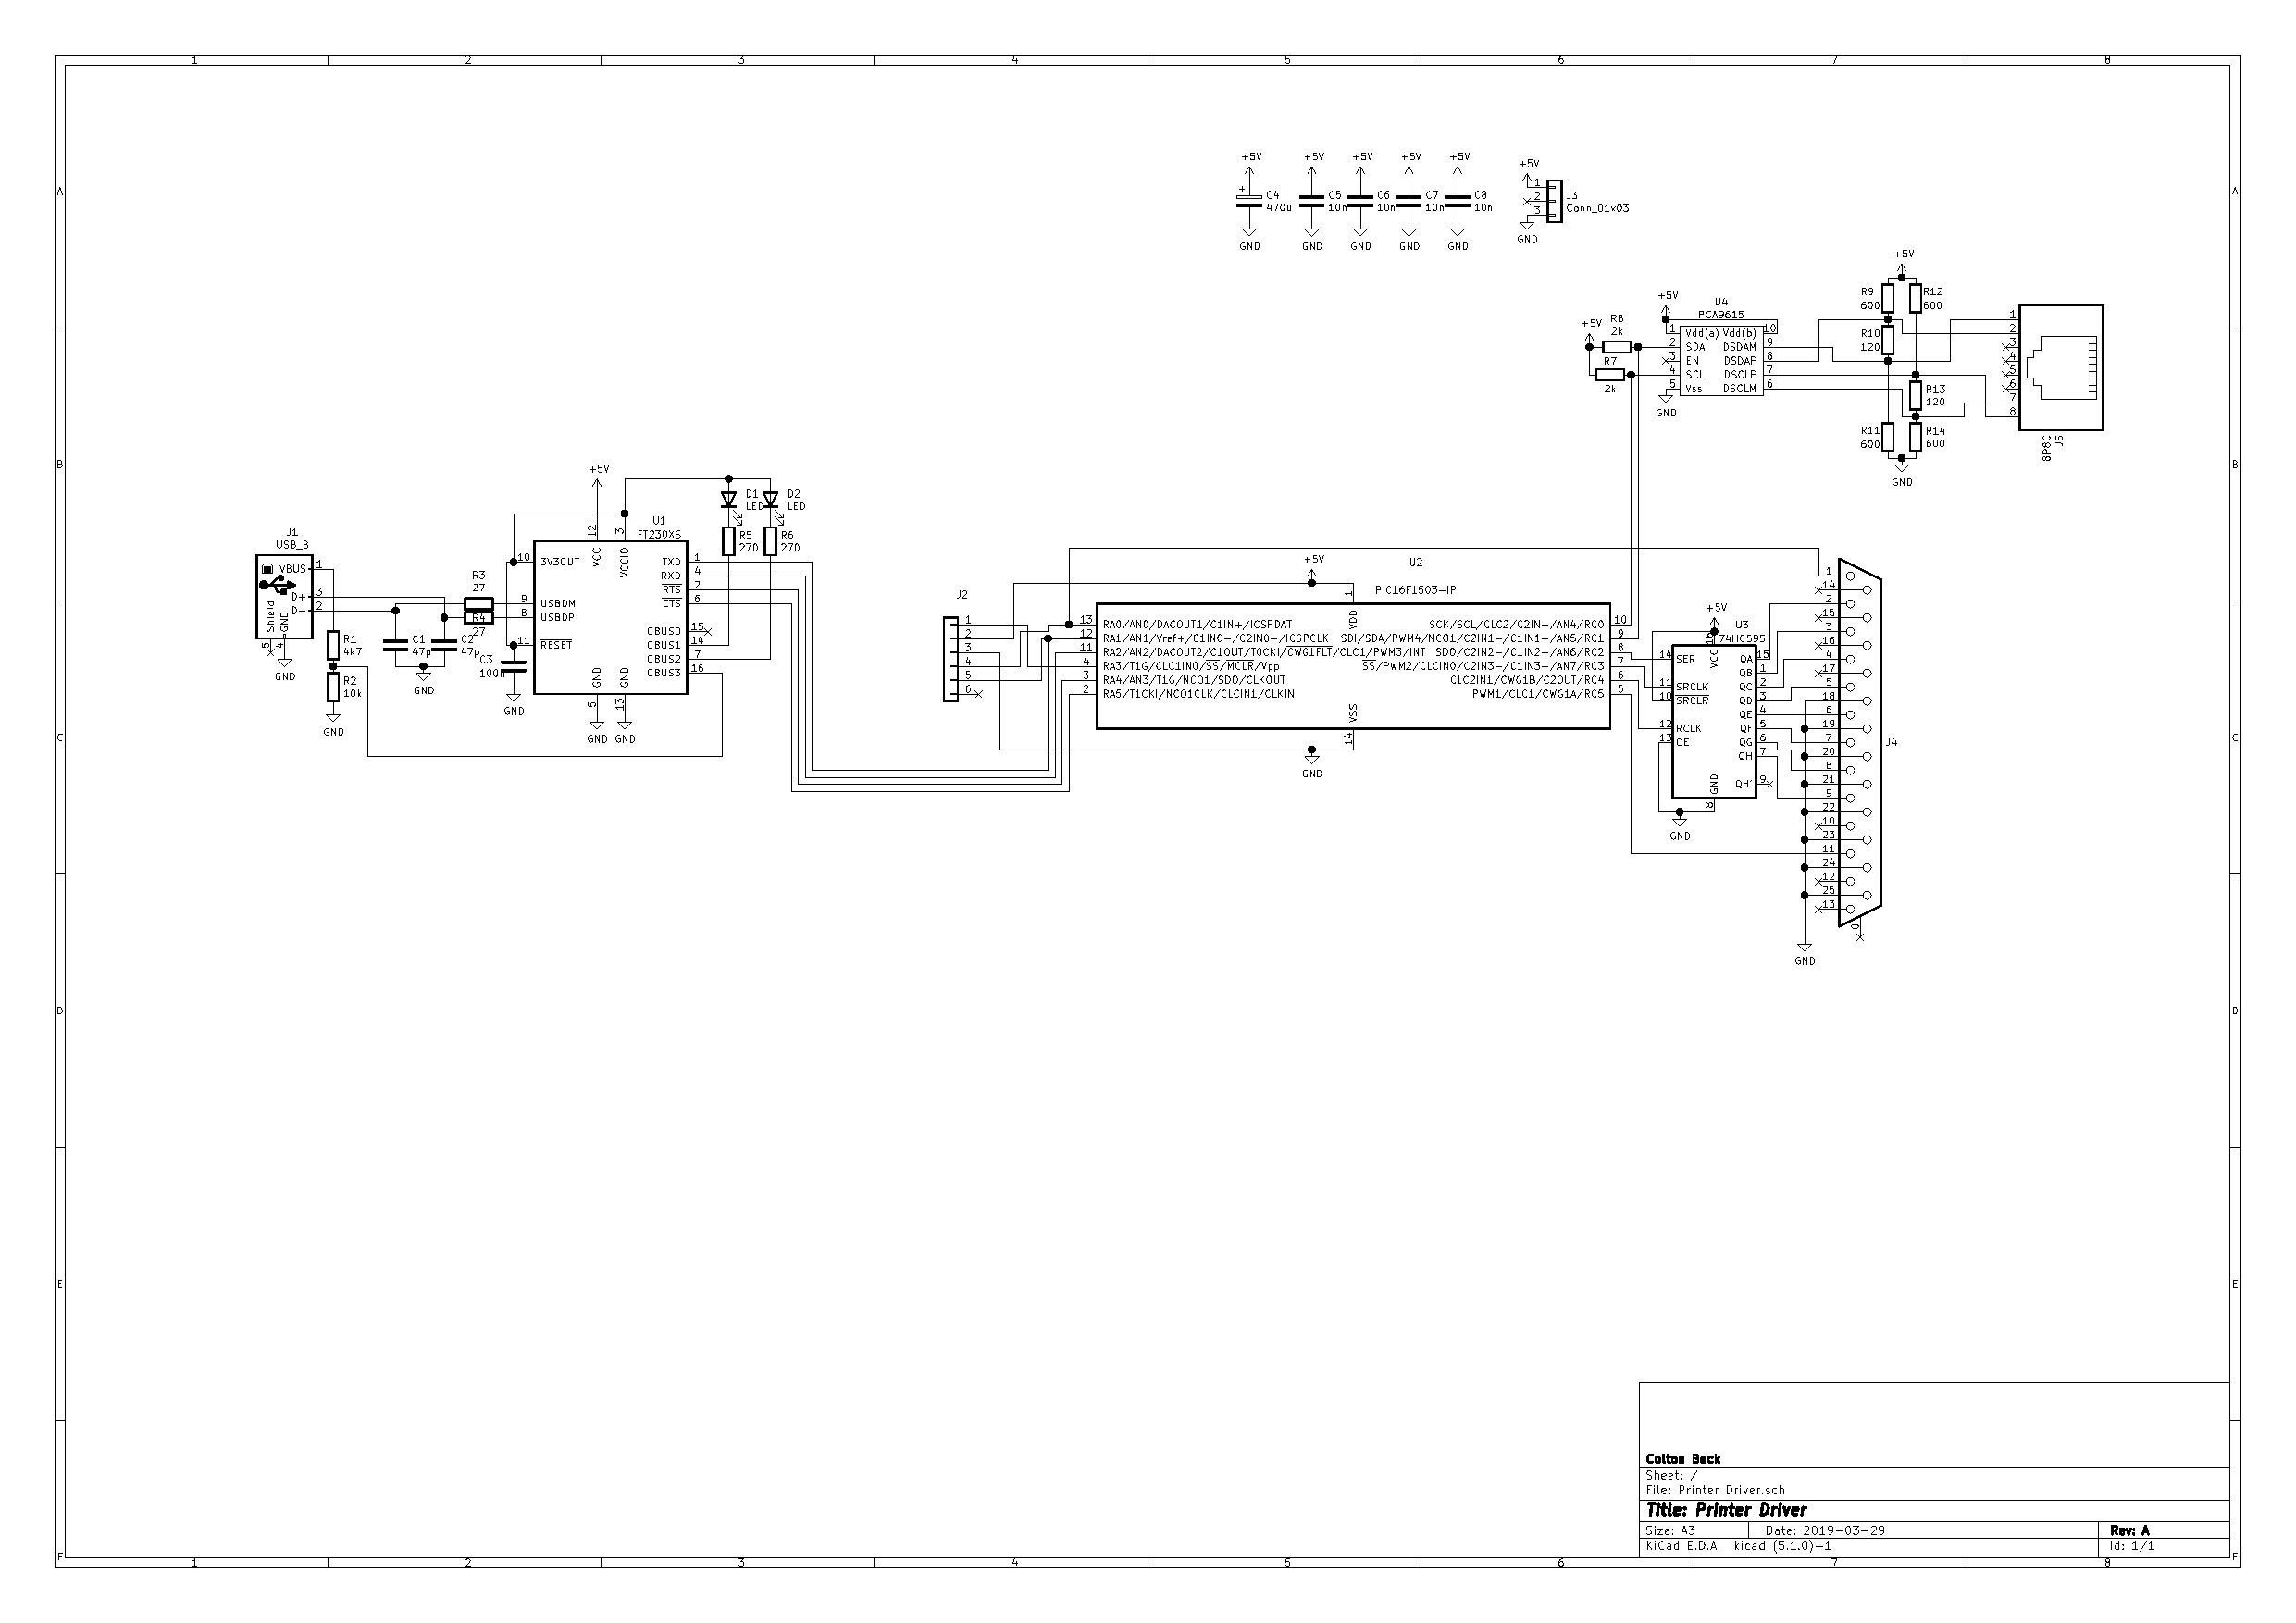
\includegraphics[height=1.1\textwidth]{../Board_Layouts/Printer_Driver/Printer_Driver.pdf}
\end{sideways}
\clearpage

\section{Card Punch \& Reader Driver Board}
\clearpage

\section{Paper Tape Punch \& Reader Driver Board}

\chapter{PCB Masks}
\section{Main Board}
\clearpage

\section{Front Panel}
\clearpage

\section{VGA Terminal}
\clearpage

\section{Line Printer Driver Board}
\clearpage

\section{Card Punch \& Reader Driver Board}
\clearpage

\section{Paper Tape Punch \& Reader Driver Board}

\chapter{Part Drawings}

\backmatter
\bibliographystyle{plain}
\addcontentsline{toc}{chapter}{Bibliography}
\bibliography{mainframe}
\end{document}